\chapter{Ошибки и исключения}
\label{errors-and-exceptions}
\section{Придержи коней!}
\begin{wrapfigure}{r}{0.4\linewidth}
    
\includegraphics[width=1\linewidth]{cyclist.png}
\end{wrapfigure}
Для этой главы невозможно подобрать подходящее место в книге.
К этому моменту вы изучили уже достаточно, чтобы начать натыкаться на ошибки, но ещё недостаточно, чтобы знать, как их контролировать.
По правде говоря, в этой главе мы не сможем рассмотреть все механизмы управления ошибками.
Отчасти это невозможно потому, что в Erlang существуют две главные парадигмы: функциональная и параллельная (concurrent).
О функциональной я рассказываю с самого начала книги: ссылочная прозрачность (чистота, referntial transparency), рекурсия, функции высшего порядка и т.д.
Но именно параллельная часть прославила Erlang: акторы, тысячи и тысячи параллельных (concurrent) процессов, деревья контроля и т.д.

Я считаю, что прежде чем переходить к параллельной части, совершенно необходимо изучить функциональную.
Поэтому я затрону лишь функциональное подмножество языка.
Чтобы управлять ошибками, нам нужно сначала их понять.\\
\colorbox{lgray}
{
\begin{minipage}{1.0\linewidth}
    \textbf{Замечание:} хоть Erlang и позволяет обращаться с ошибками в функциональном коде сразу несколькими способами, но чаще всего вы будете слышать, что делать ничего не нужно, а нужно позволить процессу упасть.
    Я уже намекал на это во \ref{introduction}~введении.
    Механизмы, которые позволяют вам программировать в таком стиле, находятся в параллельной части языка.
\end{minipage}
}
\section{Компиляция ошибок}
Ошибки подразделяются на множество видов: ошибки времени компиляции, логические ошибки, ошибки времени исполнения и сгенерированные ошибки.
В этом разделе я сконцентрирую внимание на ошибках времени компиляции, а о других расскажу чуть позже.

Ошибки времени компиляции чаще всего являются синтаксическими ошибками: нужно проверить наименование функций, языковые токены (скобки, квадратные скобки, точки, запятые), арность ваших функций и т.д.
Вот список некоторых часто встречающихся проблем времени компиляции и потенциальные способы их разрешения:

\blankline
\begin{minipage}{\textwidth}
\textbf{module.beam: Module name 'madule' does not match file name 'module'}\\
Имя модуля, которое вы указали в атрибуте \ops{-module} не совпадает с именем файла.
\end{minipage}

\blankline
\begin{minipage}{\textwidth}
\textbf{./module.erl:2: Warning: function some\_function/0 is unused}\\ 
Вы не проэкспортировали функцию, либо в месте её использования указано неверное имя или арность.
Возможно также, что вы записали функцию, которая больше нигде не вызывается.
Проверьте ваш код!
\end{minipage}

\blankline
\begin{minipage}{\textwidth}
\textbf{./module.erl:2: function some\_function/1 undefined}\\ 
Функция не существует.
Вы ввели неверное имя или указали неверную арность либо в атрибуте \ops{-export}, либо во время определения функции.
Это сообщение также можно увидеть, когда данная фунция не может быть скомпилирована.
Обычно такое случается из\--за какой\--либо синтаксической ошибки, например если вы забыли поставить точку в конце функции.
\end{minipage}

\blankline
\begin{minipage}{\textwidth}
\textbf{./module.erl:5: syntax error before: 'SomeCharacterOrWord'}\\ 
Эта ошибка может быть вызвана множеством причин, а именно: незакрытыми скобками, неверным завершением кортежа или выражения (когда вы, к примеру, закрыли заключительную ветку \ops{case} при помощи запятой).
Среди других причин можно выделить использование зарезервированного атома в вашем коде, либо юникодного символа, который был искажён при перекодировке (я видел и такое!)
\end{minipage}

\blankline
\begin{minipage}{\textwidth}
\textbf{./module.erl:5: syntax error before: }\\ 
Да уж, смысл сообщения не вполне очевиден.
Эта ошибка выдаётся, когда неверно завершена одна из строк.
Она является частным случаем предыдущей ошибки.
Просто будьте внимательны.
\end{minipage}

\blankline
\begin{minipage}{\textwidth}
\textbf{./module.erl:5: Warning: this expression will fail with a 'badarith' exception}\\
Всё в Erlang вертится вокруг динамической типизации, но не забывайте, что типизация также и сильная.
В этом примере у компилятора хватило сообразительности, чтобы определить, что в одном из арифметических выражений кроется ошибка (например, \ops{llama + 5}).
Впрочем, более сложные ошибки типов пройдут незамеченными.
\end{minipage}

\blankline
\begin{minipage}{\textwidth}
    \textbf{./module.erl:5: Warning: variable 'Var' is unused}\\
    Вы объявили переменную и нигде её не использовали.
    Это может оказаться ошибкой, так что перепроверьте ваш код.
    Если вы это сделали намеренно, то наверняка лучше поменять имя переменной на \ops{\strut{\_}} или поместить перед именем переменной знак подчёркивания (что\--то вроде \emph{\_Var}).
    Так следует поступить, когда вы считаете, что наличие имени улучшит читабельность кода.
\end{minipage}

\blankline
\begin{minipage}{\textwidth}
    \textbf{./module.erl:5: Warning: a term is constructed, but never used}\\
    Вы создали в одной из ваших функций кортеж, список, или анонимную функцию, которую впоследствии не связали с переменной и не использовали в качестве возвращаемого значения.
    Это предупреждение сообщает, что вы создаёте что\--либо впустую или совершили какую\--либо ошибку.
\end{minipage}

\blankline
\begin{minipage}{\textwidth}
    \textbf{./module.erl:5: head mismatch}\\
    Возможно, у вашей функции несколько заголовков с различной арностью.
    Не забывайте, что изменяя арность можно создавать разные функции с одинаковыми именами.
    В объявлении одной функции нельзя чередовать заголовки с разной арностью.
    Эту ошибку также можно встретить, когда между заголовками одной функции вставляют определение другой.
\end{minipage}

\blankline
\begin{minipage}{\textwidth}
    \textbf{./module.erl:5: Warning: this clause cannot match because a previous clause at line 4 always matches}\\
    У функции, определённой в модуле, после универсального условия указано конкретное.
    Поэтому компилятор предупреждает, что до более конкретного условия исполнение не дойдёт.
\end{minipage}

\blankline
\begin{minipage}{\textwidth}
    \textbf{./module.erl:9: variable 'A' unsafe in 'case' (line 5)}\\
    Переменная, определённая в одной из веток выражения \ops{case\ldots of}, используется вне этого выражения.
    Такое поведение считается небезопасным.
    Если вам понадобились такие переменные, их лучше объявлять при помощи конструкции \ops{MyVar = case \ldots of}\ldots
\end{minipage}

Этот перечень покрывает большинство ошибок компиляции, с которыми вы можете столкнуться на текущий момент. Их не так уж и много, поэтому зачастую сложнее всего найти ошибку, которая вызвала каскад ошибок, найденных в других функциях.
Ошибки, которые выдаёт компилятор, лучше всего исправлять в том порядке, в котором они указаны в списке, чтобы не начать исправлять ошибки, которые могут ими и не являться.
Иногда можно наткнуться и на другие сообщения, которые в список не попали.
Если вы с таким столкнулись, то напишите мне по email, и я как можно быстрее добавлю его в список вместе с комментариями.
\section{Нет, это у ТЕБЯ неправильная логика!}
\label{no-your-logic-is-wrong}
\begin{wrapfigure}{r}{0.35\linewidth}
    
\includegraphics[width=1\linewidth]{exam.png}
\end{wrapfigure}
Логические ошибки искать и отлаживать сложнее всего. Чаще всего эти ошибки делает сам программист: ветвления и условия (например if\--ы и case\--ы), в которых не учитываются все случаи, употребление умножения вместо деления и т.д.
Такие ошибки не приводят к аварийному завершению программы, но из\--за них программа может просто выдать неверные данные или работать незапланированным образом.

С такими ошибками вам придётся справляться самостоятельно, но в Erlang есть много средств, которые придут вам на помощь.
В их числе тестовые фреймворки, TypEr и Dialyzer (которые описывались в \ref{for-type-junkies}~главе о типах), \ref{debugger-chapter}~отладчик, \ref{dbg}~модуль трассировки и т.д.
Лучшая защита от таких ошибок \--- это тестирование.
В карьере любого программиста, к сожалению, таких ошибок хватит на пару дюжин книг, поэтому я не буду тратить на них много времени.
Легче сконцентрироваться на тех ошибках, которые приводят к аварийному завершению, так как момент их появления ясен, и они не всплывут на поверхность через 50 уровней вложенности.
Это соображение, как раз, и служит источником мантры: <<пусть процесс падает>>, о которой я уже несколько раз упоминал.
\section{Ошибки времени исполнения}
\label{run-time-errors}
Ошибки времени исполнения (run\--time errors) весьма разрушительно влияют на ваш код. Они приводят к аварийной ситуации.
Хотя в Erlang и существуют методы их контроля, но никогда не бывает лишним умение эти ошибки различать.
Поэтому я составил небольшой список таких ошибок с объяснением и примерами кода, который может их вызвать.

\textbf{function\_clause}
\begin{lstlisting}[style=erlang]
1> lists:sort([3,2,1]).
[1,2,3]
2> lists:sort(fffffff).
** exception error: no function clause matching lists:sort(fffffff)
\end{lstlisting}

Все охранные выражения завершились неудачей, либо для функции не сработал ни один из шаблонов для сопоставления с образцом.
\blankline

\textbf{case\_clause}
\begin{lstlisting}[style=erlang]
3> case "Unexpected Value" of
3>    expected_value -> ok;
3>    other_expected_value -> 'also ok'
3> end.
** exception error: no case clause matching "Unexpected Value"
\end{lstlisting}

Похоже, что кто\--то забыл указать шаблон в выражении \ops{case}, передал неподходящие данные, или забыл задать вариант для выбора по умолчанию.
\blankline

\textbf{if\_clause}
\begin{lstlisting}[style=erlang]
4> if 2 > 4 -> ok;
4>    0 > 1 -> ok
4> end.
** exception error: no true branch found when evaluating an if expression
\end{lstlisting}

Это сообщение очень похоже на ошибки \ops{case\_clause}. Не получается найти ветку, которая принимает значение \ops{true}.
Скорее всего, необходимо убедиться, что обрабатываются все возможные случаи, либо добавить вариант \ops{true} для выбора по умолчанию.
\blankline

\textbf{badmatch}
\begin{lstlisting}[style=erlang]
5> [X,Y] = {4,5}.
** exception error: no match of right hand side value {4,5}
\end{lstlisting}

Такие ошибки возникают в случае, когда не удаётся провести операцию сопоставления с образцом.
Скорее всего, вы пытаетесь провести невозможное сопоставление, пытаетесь связать переменную со значением во второй раз, или по обе стороны оператора \ops{\strut=} находятся неравные значения (что, в общем\--то и приводит к тому, что операция связывания завершается неудачей!).
Заметьте, что иногда эта ошибка возникает, потому что по мнению программиста переменная вида \emph{\_MyVar} означает то же самое, что и \ops{\strut\_}.
Переменные, имя которых начинается со знака подчёркивания \--- это обычные переменные.
Единственное их отличие в том, что компилятор не генерирует предупреждение, если эти переменные не используются после объявления.
Их можно связать со значением лишь один раз.
\blankline

\textbf{badarg}
\begin{lstlisting}[style=erlang]
6> erlang:binary_to_list("heh, already a list").
** exception error: bad argument
    in function  binary_to_list/1
        called as binary_to_list("heh, already a list")
\end{lstlisting}

Эта ошибка похожа на \ops{function\_clause} тем, что она сообщает о вызове функции с некорректными аргументами.
Главное отличие в том, что ошибка генерируется программистом, который проверяет аргументы в теле функции, а не в охранных выражениях (стражах).
Чуть позже в этой главе я покажу как генерировать такие ошибки.
\blankline

\textbf{undef}
\begin{lstlisting}[style=erlang]
7> lists:random([1,2,3]).
** exception error: undefined function lists:random/1
\end{lstlisting}
Ошибка генерируется, когда вы пытаетесь вызвать несуществующую функцию.
Убедитесь, что функция экспортируется из модуля с правильной арностью (если вы вызываете её вне модуля), и перепроверьте правильность написания имени функции и модуля.
Ещё одной причиной получения этого сообщения может служить то, что модуль находится вне пути поиска Erlang.
По умолчанию поиск происходит в текущей директории. Добавлять пути можно при помощи функции \ops{code:add\_patha/1} или \ops{code:add\_pathz/1}.
Если ничего из перечисленного не помогает, то сперва убедитесь, что модуль скомпилирован!
\blankline

\textbf{badarith}
\begin{lstlisting}[style=erlang]
8> 5 + llama.
** exception error: bad argument in an arithmetic expression
    in operator  +/2
        called as 5 + llama
\end{lstlisting}

Это сообщение появляется, когда вы пытаетесь выполнить несуществующее арифметическое действие.
Например, делите на ноль или пытаетесь выполнять арифметические операции между атомами и числами.
\blankline

\textbf{badfun}
\begin{lstlisting}[style=erlang]
9> hhfuns:add(one,two).
** exception error: bad function one
in function  hhfuns:add/2
\end{lstlisting}
Чаще всего причиной возникновения этой ошибки становится попытка использовать переменные в качестве функций, но при этом переменные функций не содержат.
В приведённом выше примере я использую функцию \ops{hhfuns} из предыдущей главы \ref{higher-order-functions}~и при этом передаю в качестве параметров\--функций пару атомов.
Такой код не сработает, и будет выброшена ошибка \ops{badfun}.
\blankline

\textbf{badarity}
\begin{lstlisting}[style=erlang]
10> F = fun(_) -> ok end.
#Fun<erl_eval.6.13229925>
11> F(a,b).
** exception error: interpreted function with arity 1 called with two arguments
\end{lstlisting}
Ошибка \ops{badarity} \--- это частный случай ошибки \ops{badfun}. 
Она происходит, когда вы используете функции высшего порядка, которым передаёте больше (или меньше) аргументов, чем они требуют.
\blankline

\textbf{system\_limit}

Есть много причин, по которым может быть сгенерирована ошибка \ops{system\_limit}: слишком много процессов (мы до них ещё доберёмся), слишком длинные атомы, у функции слишком много аргументов, количество атомов слишком велико, слишком много подсоединённых узлов и т.д.
Полный список можно прочитать в \href{http://www.erlang.org/doc/efficiency_guide/advanced.html#id2265856}{Erlang Efficiency Guide} в разделе о системных ограничениях (system limits).
Примите к сведению, что некоторые из этих ошибок настолько серьёзны, что могут привести к аварии всей виртуальной машины.

\section{Вызываем исключения}
\label{raising-exceptions}
Чтобы следить за исполнением кода и защититься от логических ошибок, иногда полезно провоцировать аварийную остановку во время исполнения кода, чтобы как можно раньше выявить возможные проблемы.
В Erlang существуют три вида исключений: \emph{ошибки (errors)}, \emph{броски (throws)} и \emph{завершения (exits)}. Все они используются в разных случаях (ну или почти в разных):

\begin{wrapfigure}{r}{0.35\linewidth}
    
\includegraphics[width=1\linewidth]{stop.png}
\end{wrapfigure}

\subsection{Ошибки}
\label{errors}
Вызов \ops{erlang:error(Reason)} завершит исполнение в текущем процесе и, после того как исключение будет поймано, предоставит трассировку стека и список аргументов для последних вызовов функций.
Это тот самый вид исключений, который вызывает ошибки времени исполнения, о которых я упоминал выше.

При помощи ошибок (errors) можно останавливать исполнение кода, в случае когда вызываемый код определённо не сможет справиться с той ситуацией, в которую он попадёт после вызова.
Если вам была возвращена ошибка \ops{if\_clause}, что вы сделаете?
Измените код, перекомпилируете его \--- вот и всё что вы можете (ну, ещё можно отобразить красивое сообщение об ошибке).
Как пример того, где не следует использовать ошибки, можно упомянуть наш модуль для работы с деревьями из главы о рекурсии \ref{recursion}.
Поиск по дереву, реализованный в модуле, не сможет найти ключ, которого в дереве нет.
В такой ситуации можно было бы ожидать, что с неизвестным результатом разберётся сам пользователь. 
Он сможет использовать значение по умолчанию, удалить дерево.
А может быть он просто проверял, есть ли в дереве какой\--либо ключ, чтобы добавить новый и т.д.
Здесь вместо вызова ошибки лучше было бы возвратить кортеж \ops{\{ok, Value\}}, или атом \ops{undefined}.

Но область применения ошибок не ограничивается лишь этими примерами.
Можно также определить собственный вид ошибок:
\begin{lstlisting}[style=erlang]
1> erlang:error(badarith).
** exception error: bad argument in an arithmetic expression
2> erlang:error(custom_error).
** exception error: custom_error
\end{lstlisting}

В этом примере оболочка Erlang не распознала \ops{custom\_error} и не вывела сообщение вида ``bad argument in \ldots'', но тем не менее эту ошибку можно использовать и обрабатывать так же как обычно (скоро мы увидим как это делать).

\subsection{Завершения}
\label{exits}
Существует два вида завершений: 'внутренние' (internal) и 'внешние' (external).
Внутренние завершения выполняются посредством вызова функции \ops{exit/1} и приводят к остановке текущего процесса.
Внешние завершения выполняются функцией \ops{exit/2} и имеют отношение к множеству процессов, принадлежащих к параллельной (concurrent) части Erlang; поэтому здесь мы сосредоточимся на внутренних завершениях, а к внешним обратимся чуть позже.

Внутренние завершения очень похожи на ошибки (errors).
На самом деле, раньше они были одним целым в составе функции \ops{exit/1}.
Использовали их в приблизительно тех же случаях.
Так как же определить, что использовать в конкретной ситуации?
Принцип выбора неочевиден.
Чтобы понять, когда нужно использовать ту или иную конструкцию, ничего не остаётся кроме как начать постепенно знакомиться с концепциями акторов и процессов.

Во введении я сравнивал процессы с людьми, которые общаются посредством почты. К этой аналогии, в общем\--то, добавить нечего, поэтому перейду к диаграммам и кружкам.
\begin{figure}[h!]
    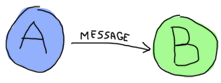
\includegraphics[width=0.4\textwidth]{a-b-msg.png}
\end{figure}

Эти процессы могут посылать друг другу сообщения.
Процесс также может ожидать прихода каких\--либо сообщений.
Можно выбирать, какие сообщения нужно ждать, какие отклонять, а какие игнорировать, через какой период времени прекращать ожидание и т.д.
\begin{figure}[h!]
    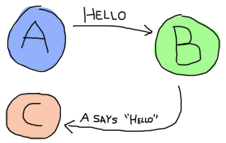
\includegraphics[width=0.4\textwidth]{a-b-c-hello.png}
\end{figure}

Эти основные концепции позволяют создателям Erlang использовать особенный вид сообщений, при помощи которых между процессами передаются исключения.
Они работают как своего рода <<последний вздох>> процесса; их посылают прямо перед тем, как процесс умирает и его код перестаёт выполняться.
Другие процессы, которые ожидали этот вид сообщений, смогут узнать об этом событии и распорядиться этим знанием как угодно.
Сделать запись в журнале, перезапустить умерший процесс и т.д.
\begin{figure}[h!]
    
\includegraphics[width=0.4\textwidth]{a-b-dead.png}
\end{figure}

Ну а теперь, когда мы имеем представление об этой концепции, нам будет проще понять разницу между \ops{erlang:error/1} и \ops{exit/1}.
Обе функции можно использовать очень похожим способом, но настоящая разница заключается в нашем намерении.
После получения такой ошибки можно решить, была ли это <<просто>> ошибка или ошибка из\--за которой стоит убить текущий процесс.
Это соображение подкрепляется тем, что функция \ops{erlang:error/1} возвращает трассировку стека, а \ops{exit/1} этого не делает.
Если бы ваша трассировка стека была достаточно велика, или у текущей функции было бы много аргументов, то отсылка сообщений о завершении каждому процессу, который ожидает такое сообщение, означало бы, что эти данные необходимо копировать. В некоторых случаях это может оказаться непрактичным.
\subsection{Броски}
\label{throws}
Броски \--- это класс исключений, используемых в случаях, которые должен обрабатывать сам программист..
По сравнению с завершениями  или ошибками, броски не имеют коннотации <<роняй процесс!>>.
Они больше относятся к управлению логикой программы.
Когда вы используете броски и ожидаете, что их будет обрабатывать программист, не лишним будет задокументировать этот факт в модуле, который их содержит.

Синтаксис бросков следующий:
\begin{lstlisting}[style=erlang]
1> throw(permission_denied).
** exception throw: permission_denied
\end{lstlisting}
\ops{permission\_denied} можно заменить чем угодно (даже сообщением \ops{'всё в порядке'}, но оно вряд ли окажется полезным для кого\--либо, а вот друзей с таким кодом вы точно не приобретёте).

Броски также можно использовать для нелокального возврата из глубокой рекурсии.
Можно привести модуль \ops{\href{http://erldocs.com/R15B/ssl/ssl.html}{ssl}} в качестве примера.
Он использует функцию \ops{throw/1} для того, чтобы протолкнуть кортежи \ops{\{error, Reason\}} назад вызывающей функции.
В свою очередь, она просто возвращает кортеж пользователю.
Благодаря этому разработчик может писать код, который рассматривает только благополучные варианты развития событий, а все исключения обрабатывает лишь в одной вышестоящей функции.

Ещё одним примером может послужить модуль для работы с массивами, в котором есть функция поиска.
В случае, если нужный элемент не был найден, эта функция возвращает значение по умолчанию, предоставленное пользователем.
Когда элемент не удаётся найти, в исключении бросается значение \ops{default}, которое обрабатывает вышестоящая функция и заменяет на пользовательское значение по умолчанию.
Это избавляет программиста модуля от необходимости передавать значение по умолчанию в каждую функцию алгоритма поиска и позволяет сконцентрироваться лишь на благополучных исходах.

Чтобы облегчить отладку кода, старайтесь использовать броски для нелокальных возвратов только в одном модуле.
К тому же, это позволит изменять внутреннее устройство модуля без необходимости менять его интерфейс.
